\documentclass[12pt]{article}
\usepackage{amsmath}
\usepackage{listings}
\usepackage{xcolor}
\usepackage{float}
\usepackage{url}
\usepackage{amsmath}
\usepackage{fancyhdr}
\usepackage{setspace} % Paket für Zeilenabstand

\pagestyle{fancy}
\fancyhf{}
\chead{\thepage} % Seitenzahl zentriert oben
\renewcommand{\headrulewidth}{0pt} % Keine Kopfzeilenlinie

\newcommand{\bracenom}{\genfrac{\lbrace}{\rbrace}{0pt}{}}

\definecolor{codegreen}{rgb}{0,0.6,0}
\definecolor{codegray}{RGB}{4,118,219}
\definecolor{codepurple}{rgb}{0.58,0,0.82}
\definecolor{backcolour}{RGB}{0,27,51}
\definecolor{textcolour}{RGB}{38, 149, 245}



\lstdefinestyle{mystyle}{
    backgroundcolor=\color{backcolour},   
    commentstyle=\color{codegreen},
    keywordstyle=\color{magenta},
    numberstyle=\tiny\color{codegray},
    stringstyle=\color{codepurple},
    basicstyle=\ttfamily\color{textcolour}\footnotesize,
    breakatwhitespace=false,         
    breaklines=true,                 
    captionpos=b,                    
    keepspaces=false,                 
    numbers=left,                    
    numbersep=5pt,                  
    showspaces=false,                
    showstringspaces=false,
    showtabs=false,                  
    tabsize=2
}



\usepackage{setspace}
\onehalfspacing
%\doublespacing

\lstset{literate=%
    {Ö}{{\"O}}1
    {Ä}{{\"A}}1
    {Ü}{{\"U}}1
    {ß}{{\ss}}1
    {ü}{{\"u}}1
    {ä}{{\"a}}1
    {ö}{{\"o}}1
    {~}{{\textasciitilde}}1
}

\lstset{style=mystyle}

    \title{\textbf{Bachelorarbeit}}
    \author{Jan Philipp Fortowski}
    \date{xx.xx.2024}
    
    \addtolength{\topmargin}{-3cm}
    \addtolength{\textheight}{3cm}
\usepackage{graphicx}

\usepackage[left=4.5cm, right=1.5cm, top=3cm, bottom=2.5cm]{geometry}
\setstretch{1.5} % Zeilenabstand von 1,5
\setcounter{page}{-1}
\begin{document}


\maketitle
\thispagestyle{empty}
\cleardoublepage
% \phantomsection
\tableofcontents
\thispagestyle{empty}
\cleardoublepage
% \phantomsection



\section{Fully Connected Layer / Feed Forward Layer}
In diesem Kapitel werden die Fully Connected Layer betrachtet, welche genau so aufgebaut sind, wie bei den Feed Forward Networks. genau genommen wird im Prinzip einfach ein Feed Forward network am Ende des Convolutional networks eingesetzt, denn die Fully Connected layer werden nur am Ende benutzt. Wenn in einem netzwerk nur die Fully Connected Layer verwendet werden, dann handelt es sich um ein Feed Forward Network. 
Das Grundprinzip ist vergleichbar kompliziert. Jede Schicht enthält sogenannte Knoten. Diese Knoten sind mit den Neuronen in einem Gehirn vergleichbar.

\begin{figure}[H]
\centering
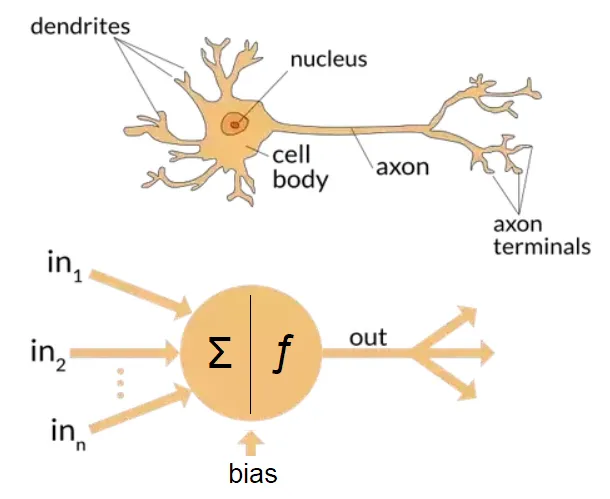
\includegraphics[scale=0.40]{./Images/BA_001_DasNeuron.png}
\caption{Das Neuron}
\label{Was kommt hier rein?}
\end{figure}

FeedForwardNetzwerk

Alle Knoten einer Schicht, sind mit allen Knoten der nächsten Schicht verbunden. Diese Verbindungen werden gewichtet, also müssen Gewichte gespeichert werden, die festlegen, wie wichtig der Input eines jeweiligen Knotens für den Aktuellen Knoten ist. Diese Knoten können angepasst werden, das heißt, dass kleine inkrementelle Anpassungen mit jeder Lern-Iteration vorgenommen werden, um das Netzwerk Stück für Stück einem Fehler-Minimum anzupassen. 

\begin{figure}[H]
\centering
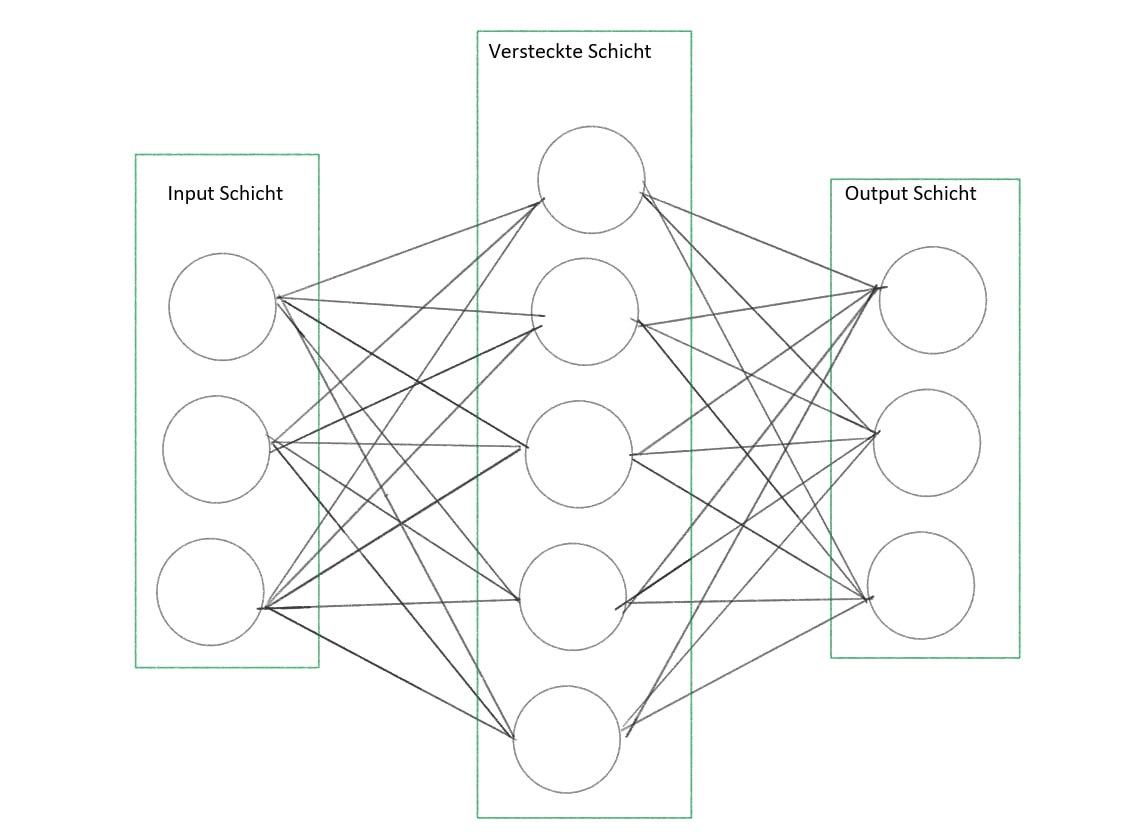
\includegraphics[scale=0.50]{./Images/BA_002_FeedForwardNetzwerk.jpg}
\caption{Das Neuron}
\label{Was kommt hier rein?}
\end{figure}

Besonders für Lineare Problemen, die nicht durch den Nullpunkt eines Koordinatensystems gehen ist es Notwendig, auch Biases mit einzurechnen. Für die Bild Erkennung ist das normalerweise nicht wichtig, und da sich die Convolutions auf die Bilderkennung Spezialisieren, wird es für dieses Projekt nicht notwendig sein, Biases einzuplanen.

In diesem Kapitel werden nun zunächst der generelle Aufbau der Klasse "FullyConnectedLayer" dargelegt, und in den beiden Unterkapiteln wird dann speziell auf den ForwardPass und auf die Backpropagation eingegangen, zusammen mit den Mathematischen Grundlagen und dem dazugehörigen Code.

Zunächst muss die Klasse erstellt werden. Die Objektvariablen sind diese:
    
\begin{lstlisting}[language=Java]
public class FullyConnectedLayer extends Layer {
    double[][] weights;
    int inLength;
    int outLength;
    double learnRate;

    private double[] lastZ;
    private double[] lastInput;
\end{lstlisting} 
in den "weights" werden die Gewichte gespeichert zwischen den Inputs und den Knoten der Schicht. Diese können angepasst werden, um den Fehler des Netzwerkes zu minimieren, damit es korrekte Klassifizierungen vornehmen kann.
Mit "inLength" ist die Menge an Inputs gemeint, das heißt zum Beispiel wie viele Pixel die Bilder haben, die in die Schicht eingespeißt werden.
Mit "outLength" entspricht dann auch der Menge an Outputs welche von der Schicht erzeugt werden, das hängt davon ab, wie viele Knoten die nächste Schicht hat, oder wenn es die letzte Schicht ist, wie viele mögliche Antworten das Netzwerk hat.
Die "learnRate" schränkt die größe der Inkremente zwischen den einzelnen gelernten Bildern ein. Dies ist Notwendig, da die berechneten inkremente, also die Steigung im Fehlergraphen, normalerweise zu groß ist, und die Fehler Minima dadurch häufig übersprungen werden. Das netzwerk soll sich aber dem Fehlerminimum annähern, also müssen die Schritte kleiner sein. Zu klein sollten sie aber auch nicht sein, weil das Netzwerk dadurch deutlich langsamer wird, und eine zu langsame Annäherung nicht Vorteilhaft ist.

%TODO Bild von Lernrate zu groß und zu klein

Mit dem Array "lastZ" und "lastInput" sollen jeweils für die Backpropagation Notwendige Zwischenschritte gespeichert werden. "lastZ" entspricht den Inputs multipliziert mit den Gewichten. Das bedeutet hierbei handelt es sich um die Ergebnisse der Schicht bevor sie durch die Activation Funktion umgerechnet werden. Mit "lastInput" sind einfach die Inputs gemeint, die zuletzt in diese Schicht geleitet wurden, und noch keinen Rechnungen unterlegen sind. Genaueres wird im Unterkapitel zur Backpropagation betrachtet, aber diese Werte sind in den verschiedenen Schritten durch die Kettenregel Notwendig.


\subsection{ForwardPass in der Fully Connected Layer}

Für den Forward Pass, also die Grundfunktion in der Querry, muss ein Array erstellt werden, welches die outputs der Schicht enthält. Beim Fully Connected Layer entspricht die menge an Outputs der menge der Knoten aus der nächsten Schicht. Ein Wert in der Output menge wird berechnet, indem jeder Input in die Schicht mit dem Gewicht multipliziert wird, welches zwischen jedem Knoten in dieser Schicht und dem Knoten der nächsten Schicht gespeichert wurde. Alle diese Werte werden dann multipliziert, und mit einer Activation Funktion umgerechnet. Dies ist dann der Output, der an die nächste Schicht übergeben wird. Hier im Code wird dieser Output durch das Array "a" dargestellt, um auf das rgebnis der Activation hinzuweisen.

Abgesehen davon werden allerdings auch noch die Werte lastInput und das Array "Z" zwischengespeichert. Diese Werte sind für die Backpropagation notwendig, daher werden die Details auch erst im nächsten Kapitel behandelt. Aber im Prinzip steht das Array "Z" für die Zwischenergebnisse, die noch mit der Activation Funktion verrechnet werden müssen. Dieses Zwischenergebnis ist für die Backpropagation wichtig, und muss daher zwischengespeichert werden.

"lastInput" ist an sich selbserklärend, hier wird einfach der letzte Input zwischengespeichert, also einfach die Werte, die bei der Querry aus der letzten Schicht eingereicht wurden, und noch nicht weiter verrechnet wurden.

\begin{lstlisting}[language=Java]
    public double[] FullyConnectedForwardPass(double[] input){
        lastInput = input;
        double[] Z = new double[outLength];
        double[] a = new double[outLength];
        //Diese schleife summiert alle Inputs auf alle outputs, und multipliziert die Inputs mit ihren jeweiligen gewichten aus der weights-Matrix
        for(int i=0; i<inLength; i++){
            for(int j=0; j<outLength;j++){
                Z[j] += input[i]*weights[i][j];
            }
        }
        
\end{lstlisting}
Nach dieser Schleife sind die Inputs mit den Gewichten verrechnet, aber die Activation Funktion wurde noch nicht angewendet. Also sollten diese Werte unter "lastZ" zwischengespeichert werden.
\begin{lstlisting}[language=Java] 
        lastZ = Z;
		
		//Diese Schleife wendet auf alle Outputs die Activation Funktion an, in diesem Falle die Sigmoid Funktion
        for(int i=0; i<inLength; i++){
            for(int j=0; j<outLength;j++){
                a[j] = Sigmoid(Z[j]);
            }
        }
        return a;
    }
\end{lstlisting} 

Der Array der zurückgegeben wird, ist der Komplette berechnete Output, und kann so an die nächste Schicht weitergeleitet werden. Im Convolutional Network kommen mehrere Schichten Fully Connected layer immer ans Ende. Die Convolution Layer und die MaxPool Layer sind auf die Erkennung von Features in Bildern und auf die Komprimierung und Verdichtung relevanter Daten in den Bildern Spezialisiert. Daher macht es keinen Sinn, diese Schichten nach einem Fully Connected Layer einzusetzten. Das Bild kann aus den Ausgaben einer Fully Connected Layer nicht wieder rekonstruiert werden, und ist daher für die anderen Schichten nicht mehr nutzbar. Es kann also davon ausgegangen werden, dass nach einem Fully Connected Layer nur noch weitere Fully Connected Layer auftreten werden. 
Außerdem soll hier angemerkt werden, dass die Convolution und Pool Layer zwar die Bilderkennung Positiv beeinflussen, simple Netzwerke bereits rein und ausschließlich mit Fully Connected Layeren aufgebaut werden können. Diese sind zwar sehr anfällig auf leichte Veränderunegn der Inputs, und die Genauigkeit lässt daher ein wenig zu wünschen übrig, aber durchaus verlässliche Ergebnisse können damit schon erzielt werden.

Da die Outputs der Fully Connected Layer keine direkten rückschlüsse auf die Bilder zulassen, die zu Anfang in das netzwerk gegeben werden, wird bei den in der Abstrakten Klasse definierten Methoden zur Rückgabe der verschiedenen Parameter auch anders verfahren, als in den anderen Layer Klassen. Die anderen Layer Klassen müssen Auskunft darüber geben können, wie viele Output Bilder sie erzeugen, und welche Dimensionen diese besitzen. Zum Beispiel gibt die Max Pool Layer zwar komprimierte Bilder zurück, das heißt dass die Dimensionen kleiner geworden sind. Allerdings werden alle Bilder, die in die Schicht eintreten, mit jedem Filter Fenster verrechnet, welches die Schicht besitzt. Das heißt die menge der Output Bilder ist die Menge der Input Bilder mal die Menge der Filter. Diese Informationen sind für die nachfolgenden Schichten von großem Wert. Bei den Fully Connected layern können nur Fully Connected layer folgen, also ist auch nur die Menge der Inputs wichtig, da Fully Connected Layer die Inputs als ein einziges 1-Dimensionales Array betrachten. Also muss nur die "getOutputElements" Methode sinnvoll betrachtet werden, diese gibt einfach die "outLength" Variable zurück. Alle anderen get-Methoden können 0 zurück geben.

\begin{lstlisting}[language=Java] 
    @Override
    public int getOutputElements() {
        return outLength;
    }
\end{lstlisting} 

\subsection{Backpropagation im Fully Connected Layer}
Backpropagation ist der Prozess, den Fehler, den ein Netzwerk macht zu Quantifizieren, und dann über alle Schichten zurückzuverfolgen. Dabei wird durch das Ableiten der Fehlerfunktion festgestellt, wie die Gewichte oder andere veränderbaren Attribute angepasst werden müssen, um sich dem Fehlerminimum zu nähern. Das Fehlerminimum wird durch kleine, inkrementelle Schritte angepeilt. Diese Schrittweise Annäherung nennt man Gradient Descent. 

Das Gradient Descent Verfahren funktioniert so, dass ein gegebenes Gewicht $w^0$ in die Fehlerfunktion $C_0$ eingesetzt wird, also die Funktion, die den Fehler quantifiziert, den das Netzwerk bei der Klassifizierung eines Bildes gemacht hat. Durch die Ableitung dieser Funktion an der gegebenen Stelle, kann eine Steigung berechnet werden, welche die Richtung angibt, in die das Gewicht angepasst werden sollte, um sich dem Fehlerminimum zu nähern. 
Das heißt also, wenn 

$C_0'(w^0)>0$, dann sollte das Gewicht $w^1$ ein Stück weiter links von $w^0$ sein, und wenn

$C_0'(w^0)<0$, dann sollte das Gewicht $w^1$ ein Stück weiter rechts von $w^0$ sein.

Das lässt sich auch algorithmisch notieren:

$$w^k:=w^{k-1}-\lambda C'(w^{k-1}), k \geq 1$$

wobei $\lambda > 0$ ist, denn $\lambda$ entspricht der Learnrate, also dem Skalierungsmaß für die Inkremente, in denen die gewichte angepasst werden. Ohne das Skalierungsmaß wären die Anpassungen zu groß, und würden die Fehlertiefpunkte regelmäßig weit überspringen, anstatt sich ihnen anzunähern [1, S.114 ff.]. 

Zuerst sollte man die Fehlerfunktion betrachten. 
Es sei der letzte Output aus dem Netzwerk genannt $O_L$. Außerdem werden die Targets für das Bild benötigt. Um ein Neuronales Netzwerk zu trainieren, braucht man nicht nur die zu klassifizierenden Inputs, diese Inputs müssen auch mit Labeln versehen sein. Ein Label gibt an, was auf dem Bild zu sehen ist. Das Ziel ist es, dass das Netzwerk eine ausgabe macht, die sich möglichst wenig von dem Label unterscheidet. Hier kommen die targets ins Spiel. Im Prinzip erstellt man ein Array, welches für jede Antwortmöglichkeit des Netzwerkes ein Feld besitzt. Das Feld, das dem label entspricht, wird auf 1 gesetzt, alle anderen Felder werden auf 0 gesetzt. Dies sind die Targets $T$.
Um nun die Loss Funktion, also die Fehlerfunktion zu berechnen, müsste man nur die Targets von den Outputs abziehen, allerdings müssen die Ergebnisse noch Quadriert werden. Das hat zwei Vorteile, der erste Vorteil ist, dass Fehler dadurch betont werden. Große Fehler haben dadurch einen noch größeren einfluss. Das hilft, sich nicht zu schnell oder zu langsam dem Fehlerminimum anzupassen. Der zweite Vorteil ist der dass durch das Quadrieren alle Fehler Positiv werden. Alle Fehler müssen nachher summiert werden. Wenn es Positive und negative Fehler gibt, würden sich diese gegenseitig aufheben. 
Alles in allem sieht die Fehlerfunktion für dieses Netzwerk dann so aus:

$$C_0 = (O_L - T)^2$$

Nun gilt es, herauszufinden, wie sich die Fehlerfunktion ändert, im Bezug auf die Gewichte und anderen veränderbaren Parameter im Netzwerk.

Dazu kann man Notieren dass die Ableitung von $C_0$ gesucht ist, im Bezug auf eine Änderung an $w_L$, damit gemeint sind die Gewichte aus der letzten Schicht.

$$\frac{\delta C_0}{\delta w_L}$$

Diese Ableitung lässt sich dank der Kettenregel weiter aufschlüsseln, sodass einzelne Komponenten entstehen, die mit Code berechnet werden können.

$$\frac{\delta C_0}{\delta w_L}=
\frac{\delta Z_L}{\delta w_L}*
\frac{\delta a_L}{\delta Z_L}*
\frac{\delta C_0}{\delta a_L}$$

Diese Terme können einzeln entschlüsselt und im Code verwendet werden. Der erste Term ist

$$\frac{\delta Z_L}{\delta w_L}$$

und beschreibt die Ableitung der Berechnung in den Knoten bevor die Transferfunktion, also zum Beispiel die Sigmoid Funktion eingesetzt wurde, im Bezug zu den Gewichten der letzten Schicht.
Diese Berechnung sieht erst einmal so aus:
Jede Schicht besitzt eine Menge an Knoten, die den Neuronen des Gehirns nachempfunden sind. Ein Knoten ist mit allen Inputs verknüpft, also mit dem Bild das in die erste Schicht geleitet wird, oder alle ausgaben der vorrigen Schicht, wenn es sich nicht um die erste Schicht handelt. Diese Verbindungen sind gewichtet, um die stärke der Synaptischen Verknüpfung zwischen den Neuronen darzustellen. Diese Gewichte werden bei der Backpropagation angepasst. Im Netzwerk werden die Gewichte in einer Matrix gespeichert, hier heißt sie "weights". 
Um einen einzelnen Knoten k zu berechnen iteriert man über alle Inputs, multipliziert diese mit dem jeweiligen Gewicht zwischen dem input und dem Knoten, also $w_{ik}$, und summiert die Ergebnisse:


$$Z_{Lk}=\sum_{i = 1}^{n}w_{ik}*x_i$$

Im Prinzip muss also nur der Term $w_{ik}*x_i$ im Bezug auf die Gewichte abgeleitet werden, um die Änderungsrate berechnen zu können, wenn die Gewichte angepasst werden.

$$\frac{\delta Z_L}{\delta w_L}=x_i$$

Wie wir sehen entspricht x einfach den Inputs aus der vorigen Schicht. Diese sollten also beim Forwardpass auf jeden Fall immer zwischengespeichert werden, im hier in der Backpropagagtion benutzt werden zu können. Dies wurde im letzten Kapitel schon vorbereitet.

Der nächste Term 
$$\frac{\delta a_L}{\delta Z_L}$$ Beschäftigt sich mit dem Einfluss von $Z_L$ auf die Ableitung von der Activation Funktion. Es gibt verschiedene Transferfunktionen $T(x)$, und zwei werden besonders häufig verwendet. Zum einen die Sigmoid Funktion, zum anderen ReLu. 
ReLu ist besonders leicht zu berechnen, und wird daher für schnelleres Lernen eingesetzt. Alle Werte unter 0 werden zu 0 Transformiert und ausgegeben, alle Werte über 0 werden so zurückgegeben, wie sie sind.

$$
T(x):=
\left\{
\begin{tabular}{l}
0 für $x<0$ \\
x für $x\geq 0$
\end{tabular}
\right\}
:=T_1(x)
$$

Die Ableitung davon ist auch denkbar einfach, Unter 0 hat die x keinen einfluss, über 0 hat es einen direkten einfluss, also 1.

$$
T'(x):=
\left\{
\begin{tabular}{l}
0 für $x<0$ \\
1 für $x\geq 0$
\end{tabular}
\right\}
:=T'_1(x)
$$

Etwas aufwändiger ist die Sigmoid Funktion, die auch in diesem Netzwerk verwendet werden soll. Die Sigmoid Funktion sieht so aus:

$$\sigma (x)=\frac{1}{(1+e^{-x})}$$
Und ihre Ableitung:
$$\sigma '(x)=\sigma (x)(1-\sigma(x))$$

%TODO Es kann hier noch die Ableitung der Sigmoid erklärt werden, so wie Prof Lanz sich das gewünscht hat. Allerdings ist dies Extrem aufwändig, und nicht zu empfehlen...

Hier ist der Code für die Sigmoid Funktion und ihre Ableitung:
\begin{lstlisting}[language=Java] 
    //Die Sigmoid Funktion
    public double Sigmoid(double weightedInput) {
        return 1.0 / (1 + Math.exp(-weightedInput));
    }
    //Die Ableitung der Sigmoid Funktion
    public double SigmoidAbleitung(double weightedInput) {
        double activation = Sigmoid(weightedInput);
        return activation * (1.0 - activation);
    }
    
\end{lstlisting} 

Und hier ist die Relu Funktion mit ihrer Ableitung. Im Code sehr einfach umzusetzen:

\begin{lstlisting}[language=Java] 
    //Die ReLu Funktion
    public double ReLu(double weightedInput) {
        if (weightedInput <= 0)
        return 0.0;
    else
        return weightedInput;
    }
        
    //Die Ableitung der ReLu Funktion
    public double ReLuAbleitung(double weightedInput) {
        if (weightedInput <= 0)
            return 0.01; //Leak Value, um Tote bereiche zu vermeiden. Vermutlich bei Sigmoid kein Problem
        else
            return 1.0;
    }
\end{lstlisting} 

Nun kommen wir zum vorerst letzten Term:

$$\frac{\delta C_0}{\delta a_L}$$

gesucht ist die Ableitung der Cost oder Fehlerfunktion, im Bezug auf die Outputs der letzten Schicht im Netzwerk. Dies ist die Fehlerfunktion:

$$C_0 = (O_L - T)^2$$

Hierbei ist $O_L$ gleich $a_L$ des Netzwerkes.
Die Ableitung hier ist einfach:

$$\frac{\delta C_0}{\delta O_L} = 2(O_L - T)$$

Damit sind alle Terme der letzten Schicht im Netzwerk geklärt, und können eingesetzt werden.
Um im Code nachvollziehen zu können, welcher Wert was macht, nennen wir die Werte einfach genau so, wie sie geschrieben werden.


$$\frac{\delta Z_L}{\delta w_L} \rightarrow dZdw $$ \\
$$\frac{\delta a_L}{\delta Z_L} \rightarrow dadZ $$ \\
$$\frac{\delta C_0}{\delta a_L} \rightarrow dCda $$ \\

nachdem die Namenskonvention geklärt ist, kann der Code erstellt werden:

\begin{lstlisting}[language=Java] 
    public void backPropagation2(double[] dCda) {
        double dZdw;
        double dadZ;
        double dCdw;

        for(int k=0; k<inLength; k++){
            for(int j=0; j<outLength; j++){
                dZdw = lastInput[k];
                dadZ = SigmoidAbleitung(lastZ[j]);

                dCdw = dZdw * dadZ * dCda[j];

                weights[k][j] -= dCdw*learnRate;
            }
        }
    }
\end{lstlisting} 

Um die Methode Modular zu halten, wird die Ableitung vom Error außerhalb der Methode berechnet, und als "dCda", also Ableitung der Cost Funktion im Bezug auf die Outputs der letzten Schicht, an die Methode übergeben. Dadurch wird die Backpropagation angestoßen. Als nächstes werden die Variablen aufgestellt. Das Ziel ist es, "dCdw", also die Cost Funktion im Bezug auf die Gewichte zu ermitteln. 
In einer verschachtelten Schleife über alle Gewichte werden die Variablen zunächst belegt.
Warum über alle Gewichte? Weil die Änderung für jedes Gewicht berechnet werden soll. 
"dZdw" Entspricht dem letzten Input aus der vorletzten Schicht. "dadZ" ist das Ergebnis der Ableitung der Transferfunktion, hier Sigmoid, im Bezug auf die gewichteten Inputs der vorletzten Schicht.
Um also das Ergebnis der Ableitung der Cost Funktion im Bezug auf die Gewichte der letzten Schicht im Netzwerk zu berechnen, müssen diese Zwischenergebnisse nur noch multipliziert werden. Das heißt die entsprechenden Werte von "dCda", die übergeben wurden, multipliziert mit "dZdw" und "dadZ".
Das Ergebnis dieser Rechnung ist die Steigung der Fehlerfunktion, an der Stelle, an der das jeweilige Gewicht eingesetzt wurde. Wenn die Steigung Positiv ist, sollte das Gewicht verringert werden, also abgezogen werden, um sich dem Fehlerminimum anzunähern.
Wenn die Steigung Negativ ist, liegt das Fehlerminimum voraus, also sollte das Gewicht vergrößert werden.
Wichtig an dieser Stelle ist noch zu beachten, dass die berechnete Änderungsrate zu groß ist, und mit der LearnRate multipliziert werden muss, bevor der Wert von den Gewichten abgezogen wird. Es könnte sonst dazu kommen, dass das Fehlerminimum übersprungen wird.

Dies ist de vollständige Berechnng der Anpassungs der Gewichte in der letzten Schicht. Aber wie wird nun die vorletzte Schicht angepasst? und die Schicht davor?
Im Prinzip muss der Fehler weiter durch das Netzwerk zurückgereicht werden, und in jeder Schicht, die anpassbare Parameter hat, müssen diese Parameter so angepasst werden, wie sie für den Fehler verantwortlich waren.

Dies kann vollständig modular aufgebaut werden, sodass eine völlig variable anzahl an Schichten möglich werden. Wenn man die Ableitung der Cost Funktion im Bezug auf die Gewichte der letzten Schicht, und die Ableitung der Cost Funktion im bezug auf die Gewichte der Vorletzten Schicht miteinander vergleicht, so fällt auf, dass es Terme gibt, die zum Teil völlig gleich sind, das es einen term gibt der sich verändert, und dass es zwei neue Terme gibt, die sich von alten termen nur darin unterscheiden, dass sie Inputs uas der Vorletzten, anstatt aus der letzten Schicht benötigen.

Diesmal wird die Änderungsrate der Cost Funktion $C$ gesucht, in Abhängigkeit von den Gewichten der vorletzten Schicht, $w_{(L-1)}$.

$$\frac{\delta C_0}{\delta w_{(L-1)}}=
\frac{\delta Z_{(L-1)}}{\delta w_{(L-1)}}*
\frac{\delta a_{(L-1)}}{\delta Z_{(L-1)}}*
\frac{\delta Z_L}{\delta a_{(L-1)}}*
\frac{\delta a_L}{\delta Z_L}*
\frac{\delta C_0}{\delta a_L}*
$$

Die letzten beiden Terme sind schon aus der vorherigen Rechnung bekannt.

$$\frac{\delta a_L}{\delta Z_L}$$
$$\frac{\delta C_0}{\delta a_L}$$

Damit gemeint sind die Ableitung der Cost Funktion, sowie die Ableitung der Activation Funktion. Diese können bereits in der Letzten Schicht verrechnet werden, und an die vorletzte Schicht übergeben werden. Außerdem kann die Ableitung des Dritten Terms ebenfalls in der letzten Schicht berechnet und übergeben werden. Dieser Unterscheidet sich von dem dritten Term in den Berechnungen für die letzte Schicht. Anstatt die Änderungsrate im Bezug auf Änderungen an den Gewichten, berechnet dieser Term im Bezug auf die Änderungen an den Inputs aus der vorherigen Schicht.

$$\frac{\delta Z_L}{\delta a_{(L-1)}}$$

Die Ableitung der Berechnung der Gewichteten Outputs der letzten Schicht, im Bezug auf die Inputs der vorletzten Schicht. Die Änderungsrate hängt hierbei völlig von den Gewichten der letzten Schicht ab, also gilt:

$$\frac{\delta Z_L}{\delta a_{(L-1)}} = w_L$$

Wenn diese drei Terme bereits in der Letzten Schicht berechnet werden, können sie ohne weiteres an die vorletzte Schicht übergeben werden. Nach diesem Prinzip können beliebig viele Schichten aneinander gereiht werden, und sich gegenseitig ihre berechneten Werte durchreichen. 

Die bisherigen Werte kann man zusammenfassen:

$$
\frac{\delta Z_L}{\delta a_{(L-1)}}*
\frac{\delta a_L}{\delta Z_L}*
\frac{\delta C_0}{\delta a_L}
= \frac{\delta C_0}{\delta a_{(L-1)}}
$$

$\frac{\delta C_0}{\delta a_{(L-1)}}$ kann einfach an die nächste Backpropagation Methode übergeben werden.

Dort, in der vorletzten Schicht, wird das gleiche getan, wie zuvor in der Letzten Schicht. Die Eingabe, "dCda", wird mit diesen Termen verrechnet:

$$
\frac{\delta Z_{(L-1)}}{\delta w_{(L-1)}}*
\frac{\delta a_{(L-1)}}{\delta Z_{(L-1)}}*
\frac{\delta C_0}{\delta a_{(L-1)}}
$$

Diese Terme sind im Prinzip die gleichen wie zuvor, nur auf die aktuelle Schicht gemünzt. 

Um eine kleine Zusammenfassung zu schaffen:

Jede Schicht muss 3 Terme miteinander multiplizieren. 

Der erste Term beschreibt die ableitung der Cost Funktion im Bezug auf die Outputs der aktuellen Schicht. Bei der letzten Schicht im Netzwerk, also der ersten Schicht im Backpropagation Verfahren, ist das einfach die Ableitung der Cost Funktion, welche zum berechnen die Outputs des Netzwerks, und die erwarteten Werte der Inputs des Netzwerkes benötigt. In allesn weiteren Schichten handelt es sich dabei um errechnete Werte aus den anderen Schichten, welche übergeben werden. Ab hier werden sie "dCd0" genannt, da der Name "dZda" anderweitig noch gebraucht wird.

Der 2 Term sieht in jeder Schicht gleich aus, es kommt hierbei lediglich auf die Inputs an. Es handelt sich um die ableitung der Activation Funktion, im Bezug auf die Gewichteten Inputs.

$$\frac{\delta a}{\delta Z}$$

Dieser Schritt wurde zuvor schon implementiert.
Übrig bleibt also nur der letzte Term. diesen gibt es in zwei ausführungen, und zwar einmal um die Gewichte der aktuellen Schicht anzupassen, und einmal um die Werte zu berechnen, die an die nächste Schicht im Backpropagation Verfahren gereicht werden sollen.
Um die Gewichte anzupassen, benötigt man hierbei die Inputs aus der letzten Schicht, und auch dies wurde bereits Implementiert. Es bleibt nur noch die Berechnung für die nächste Schicht. Wie weiter oben schon festgestellt, handelt es sich dabei um die gewichte der Aktuellen Schicht. 
Nun zur Form. Es geht immer noch darum, die Fehler, die das Netzwerk gemacht hat, an die Schichten weiterzureichen. Daher muss ein Vektor erstellt werden, der den Outputs der vorherigen Schicht entspricht, und die Fehler enthält, die von der Schicht verursacht wurden.
Dieser Vektor wird nun als "dCda" erstellt, denn er soll immerhin die Änderngsraten enthalten, die durch die Ableitung der Cost Funktion im Bezug auf die Outputs "a" der vorherigen Schicht berechnet wurden. Eine weiter neue Variable ist der double "dZda", welcher schlichtweg das Gewicht enthält, welches gerade angepasst werden soll.

\begin{lstlisting}[language=Java]
    @Override
    public void backPropagation(double[] dCd0) {
        double[] dCda = new double[inLength];
        double dZdw;
        double dadZ;
        double dCdw;
        double dZda;
\end{lstlisting} 
In der äußeren Schleife wird nun eine Variable "dCda\_sum" geführt. In dieser werden alle Änderungsraten der Cost Funktion im Bezug auf die Inputs der letzten Schicht aufsummiert. Dieser Wert wird für jeden input der aktuellen Schicht erstellt und im Vektor "dCda" gespeichert.
\begin{lstlisting}[language=Java]  
        for(int k=0; k<inLength; k++){

            double dCda_sum = 0;

            for(int j=0; j<outLength; j++){
                dZdw = lastInput[k];
                dadZ = SigmoidAbleitung(lastZ[j]);
\end{lstlisting} 
In der inneren Schleife werden nun auch die entsprechenden Gewichte festgehalten. Wie zuvor werden nun die Änderungsraten für die aktuellen gewichte berechnet und werden angewandt.
\begin{lstlisting}[language=Java]  
                dZda = weights[k][j]; 

                dCdw = dZdw * dadZ * dCd0[j];

                weights[k][j] -= dCdw*learnRate;
\end{lstlisting} 
Zuletzt wird aber die Änderungsrate der Cost Funktion im Bezug auf die Inputs der vorherigen Schicht berechnet. Statt dem letzten Input wird hier das Aktuelle gewicht multipliziert, und zur variable "dCda\_sum" hinzugefügt.
\begin{lstlisting}[language=Java]              
                dCda_sum += dZda * dadZ * dCd0[j];
            }
            dCda[k] = dCda_sum;
        }
\end{lstlisting} 
Nach den Schleifen muss nur noch die Backpropagation Methode der vorherige Schicht aufgerufen werden, und dieser der vector "dCda" übergeben werden.
\begin{lstlisting}[language=Java]   
        if(previousLayer!= null){
            previousLayer.backPropagation(dCda);
        }
    }
\end{lstlisting} 

Dieser Prozess muss zwar noch in den anderen Layern implementiert werden, aber auf diese elegante Weise kann die Backpropagation Methode umgesetzt werden werden. Wenn man das Netzwerk ausschließlich aus Fully Connected Layern aufbaut, funktionieren klassifikatorische Aufgaben schon ganz gut. Durch Einsatz von Pooling Layern und Convolutional Layern kann die Effizienz allerdings noch weiter gesteigert werden.

\section{Pooling Layer}
Pooling Layer werden dazu verwendet, um das sogenannte Downsampling zu betreieben. Downsampling bedeutet einfach, dass eine geringere Auswahl an Daten weitergegeben werden.
In einem Netzwerk benutzt man eines dieser Verfahren, um die weiteren Schichten nur mit den nötigsten Daten zu belasten. Gerade in Anbetracht der Größe der Daten, die bei den Convolutional Layern entstehen, kann das viel Zeit sparen. Aber Hauptsächlich sorgt dies auch dafür, dass das Netzwerk weniger anfällig für Veränderungen der Daten wird. Leichte Veränderungen der Daten können für gravierende Änderungen sorgen, das heißt wenn ein Bild nicht korrekt Zentriert ist, oder wenn es um ein paar Grad gedreht wird, kommt ein Netzwerk schnell durcheinander.
Die Convolution Layer erstellen Feature Maps, in denen die Features allerdings auch die gleichen Positionen haben, wie in den Inputs. Dadurch können bei kleinen Veränderungen schon Fehler in den nächsten Schichten entstehen. Dem kann man durch das Downsampling entgegenwirken.

Auf eine Gewisse weise können die Daten bereits in den Convonlutional Layern "gedownsampelt" werden, wenn die Schrittgröße (Stride) beim anwenden der Filter Größer ist als 1.

Wie genau Funktioniert ein Pooling Layer dann? so wie bei den Convolutional Layern werden Filter eingesetzt. Diese sind aber kleiner, und funktionieren anders. Meist ist ein Filter hier nur 2x2 groß, und bei der Anwendung wird eine Schrittgröße von 2 verwendet. Die Filter überlappen die Felder nicht, die bereits behandelt wurden. 
Auf die Pixel, auf die der Filter angewandt wird, werden nun eine Pooling Operation durchgeführt. 

Zwei mögliche Pooling Operationen sind das Average Pooling und das Maximum Pooling. 
\begin{itemize}
  \item Das Average Pooling gibt den Durchschnitt aller Werte als Output zurück, während
  \item das Maximum Pooling nur den Größten Wert der betrachteten Werte zurückgibt.
\end{itemize}
Es gibt noch weitere, wie zum Beispiel das Globale Pooling, bei dem die Gesammte Feature Map auf einen einzigen Wert reduziert wird. Dadurch soll auf eine möglichst Aggressive Art festgestellt werden, ob ein bestimmtes Feature überhaupt in der Feature Map vorkommt. Je nach Anwendungsfall kann auch diese Methode Erfolg bringen.

Zunächste wird die Maximum Pooling Layer betrachtet.
genau wie bei den Convolutional Layern, wird hier eine StepSize verwendet. Zwar ändert sich diese in den meisten Fällen nicht, aber es ist gut, die Flexibilität zu haben.
Die windowSize legt fest, welche Dimensionen der Filter haben soll.
\\Außerdem ist es hilfreich, wenn die input Parameter auch gespeichert werden, damit gemeint sind input length, input rows und input columns, also die menge an Bilder, zusammen mit den Zeilen und Reihen die diese Bilder haben.

\begin{lstlisting}[language=Java]
public class MaxPoolLayer extends Layer {

    private int stepSize;
    private int windowSize;

    private int inLength;
    private int inRows;
    private int inCols;
\end{lstlisting} 

\subsection{Forward Propagation im Pooling Layer}
Wie oben beschrieben, wird hier ein kleiner Filter benutzt, der über die Input Bilder gleitet, und entweder den maximalen Wert, oder den Durchschnittswert zurückgibt. 

%TODO Bild einfügen

Zunächst wird eine Methode benötigt, die den Filter darstellt, und eine Feature Map durchläuft. 

\begin{lstlisting}[language=Java]
 public double[][] pool(double[][] input){
 		//Die Output Dimensionen müssen berechnet werden
        double[][] output = new double[getOutputRows()][getOutputCols()];
        //zwei Schleifen um über den Input zu Iterieren
        for(int r=0; r<getOutputRows(); r+=stepSize){
            for(int c=0; c<getOutputCols(); c+=stepSize){
                double max = 0.0;
                //Zwei Schleifen um das Maximum im Fenster des Filters zu finden
                for(int x=0; x<windowSize; x++){
                    for(int y=0; y<windowSize; y++){
                        if(max<input[r+x][c+y]){
                            max=input[r+x][c+y];
                        }
                    }
                }
                output[r][c] = max;
            }
        }
        return output;
    }
\end{lstlisting}
Alternativ kann natürlich auch der Durchschnitt errechnet und ausgegeben werden. Dazu sind keine Großen Anpassungen nötig:
\begin{lstlisting}[language=Java]
 public double[][] pool(double[][] input){
 		//Die Output Dimensionen müssen berechnet werden
        double[][] output = new double[getOutputRows()][getOutputCols()];
        //zwei Schleifen um über den Input zu Iterieren
        for(int r=0; r<getOutputRows(); r+=stepSize){
            for(int c=0; c<getOutputCols(); c+=stepSize){
                double average = 0.0;
                //Zwei Schleifen um die Werte im Fenster des Filters zu addieren
                for(int x=0; x<windowSize; x++){
                    for(int y=0; y<windowSize; y++){
                    	average+=input[r+x][c+y];
                    }
                }
                //Der Durchschnitt muss natürlich noch durch die menge der im Filter Fenster enthaltenen Pixel geteilt werden
                output[r][c] = average/(windowSize*windowSize);
            }
        }
        return output;
    }
\end{lstlisting}
Im Code wurden die Methoden getOutputRows und getOutputCols schon verwendet, also müssen diese auch noch Implementiert werden. Die Formel dazu sieht folgendermaßen [2] aus:
$$H_{out} = floor(1 + (H - pool\_height)/stride)$$
$$W_{out} = floor(1 + (W - pool\_ width)/stride)$$

$H_{out}$ und $W_{out}$ entsprechen den Dimensionen des output Fensters. 

Und im Code werden diese so umgesetzt:

\begin{lstlisting}[language=Java]
    public int getOutputRows() {
        return (inRows - windowSize) / stepSize + 1;
    }

    public int getOutputCols() {
        return (inCols - windowSize) / stepSize + 1;
    }
\end{lstlisting}

\subsection{Backpropagation im Pooling Layer}
Für die Backpropagation in einem Pooling Layer müssen keine gewichte oder Biases angepasst werden. Denn diese gibt es hier nicht. Stattdessen muss der Fehler aber trotzdem auf einen der Inputs zurückgeführt werden, das heißt zum Beispiel, dass beim Max Pooling aus jedem von dem Filter Fenster betrachteten Gebiet der Maximale Wert für den Fehler verantwortlich war, und die anderen Werte keine Verantwortung tragen. 

%TODO Bild einfügen

Am besten gelingt dies, indem die Positionen der Maximal Werte gespeichert werden.
Dazu sollten erst neuen Instanzvariablen angelegt werden:


\begin{lstlisting}[language=Java]
    List<int[][]> lastMaxRow;
    List<int[][]> lastMaxCol; 
\end{lstlisting}

Zwei Listen, welche 2-Dimensionale Arrays enthalten, jeweils eine liste für die Koordinate der X und eine für die Y Achse.
Danach müssen diese Initialisiert werden, und zwar in der "maxPoolForwardPass" Methode. Das stellt sicher, dass sie initialisiert werden, bevor das pooling beginnt:

\begin{lstlisting}[language=Java]
    public List<double[][]> maxPoolForwardPass(List<double[][]> input) {
        //Initialisierung der lastMaxRow und Col, in denen die Position der Maximalen Werte gespeichert werden
        lastMaxRow = new ArrayList<>();
        lastMaxCol = new ArrayList<>();
\end{lstlisting}

Um die Werte dann zu speichern, müssen diese während der pooling Operation gespeichert werden.
Dazu können zwei 2-Dimensionale Integer Arrays verwendet werden, welche mit den gleichen Maßen initialisiert werden, wie die Outputs. Das heißt, dass für jeden Output die X und Y Koordinate im dazugehörigen lastMax-Array ein entsprechender Platz vorhanden ist.

\begin{lstlisting}[language=Java]
public double[][] pool(double[][] input) {
        double[][] output = new double[getOutputRows()][getOutputCols()];

        int[][] maxRows = new int[getOutputRows()][getOutputCols()];
        int[][] maxCols = new int[getOutputRows()][getOutputCols()];   
\end{lstlisting}
für den Fall, das kein maximum über 0 gefunden werden konnnte, sollten Koordinaten trotzdem markiert werden, darum werden die alle Felder zuerst auf -1 gesetzt:
\begin{lstlisting}[language=Java]
        for (int r = 0; r < getOutputRows(); r += stepSize) {
            for (int c = 0; c < getOutputCols(); c += stepSize) {
                double max = 0.0;

                maxRows[r][c] = -1;
                maxCols[r][c] = -1;
\end{lstlisting}
In der inneren Schleife müssen die Koordinaten natürlich auch gespeichert werden, wenn ein neues Maximum im Fenster gefunden wurde:
\begin{lstlisting}[language=Java]
                for (int x = 0; x < windowSize; x++) {
                    for (int y = 0; y < windowSize; y++) {
                        if (max < input[r + x][c + y]) {
                            max = input[r + x][c + y];
//Koordinaten des Maximalen Wertes werden in den dafür vorgesehenen Arrays gespeichert
                            maxRows[r][c] = r + x;
                            maxCols[r][c] = c + y;
                        }
                    }
                }
                output[r][c] = max;
            }
        }
\end{lstlisting}
zuletzt müssen die Arrays, welche die Koordinaten enthalten noch den Listen hinzugefügt werden, die am Anfang Initialisiert wurden:
\begin{lstlisting}[language=Java]
        lastMaxRow.add(maxRows);
        lastMaxCol.add(maxCols);
        return output;
    }
\end{lstlisting}

Die eigentliche Umsetzung der Backpropagation findet in der "backPropagation" Methode statt. Der Grundgedanke ist der, dass nur der Maximalwert zum Fehler beigetragen hat, und daher auch nur dieser Wert angepasst werden muss. Also Erstellt man eine Fehlermatrix, die überall nur 0 enthält, außer an den Stellen, von denen die Maximalwerte genommen wurden. Da werden die Fehlerwerte eingetragen, und dann, da es hier keinerlei Gewichte oder Biases gibt, wird diese Fehlermatrix dann an die nächste Schicht weitergegeben.
Zuerst muss eine Liste mit den Fehlermatrizen erstellt und initialisiert werden und es wird ein Zähler benötigt, um über alle vorher angelegten Koordinaten-Matrizen zu iterieren, welche die Positionen der Maximalwerte enthalten.
\begin{lstlisting}[language=Java]
    public void backPropagation(List<double[][]> dLdO) {
        List<double[][]> dXdL = new ArrayList<>();
        int l=0;
\end{lstlisting}
Dann wird über alle eingehenden Fehlermatrizen iterriert, um die jeweilige Fehlermatrize zu erstellen, die an die nächste Schicht weitergegeben wird. letztere muss zunächst initialisiert werden.  
\begin{lstlisting}[language=Java]
        for(double[][] array : dLdO){
            double[][] error = new double[inRows][inCols];
\end{lstlisting}
Dann muss die eingehende Fehlermatrix durchiteriert werden. für jeden eingehenden wert wird die Position des verantwortlichen Maximalwerts ermittelt. In der entstehenden Fehlermatrix wird der eingehende fehler dann an der jeweiligen Position hinzugefügt. Wichtig ist, dass der Wert zu den bestehenden Werten hinzugefügt wird. meistens überlappen sich die betrachteten fenster in der Pooling Phase nicht, aber falls doch, kann ein ein Wert in mehreren Fenstern der Maximalwert sein, daher ist dieser wert dann auch sozusagen für mehrere Fehler verantwortlich. Das wird dadurch ausgedrückt, dass der Fehlerwert dann aufaddiert wird.
\begin{lstlisting}[language=Java]
            for(int r=0; r<getOutputRows(); r++){
                for(int c=0; c<getOutputCols(); c++){
                    int max_i = lastMaxRow.get(l)[r][c];
                    int max_j = lastMaxCol.get(l)[r][c];

                    if(max_i != -1){
                        error[max_i][max_j] += array[r][c];
                    }
                }
            }
\end{lstlisting}
Zuletzt müssen die entstandenen Fehlermatrizen nur noch der liste hinzugefügt werden, welche dann an die nächste Schicht weitergegeben wird.  
\begin{lstlisting}[language=Java]
            dXdL.add(error);
            l++;
        }
        if(previousLayer != null){
            previousLayer.backPropagation(dXdL);
        }
    }
\end{lstlisting}

Für den Fall, dass die eingehenden Fehler keine liste, sondern eine einfaches Array ist, also zum Beispiel weil die nächste Schicht eine Fully Connected Layer ist, erstellt man noch eine "backPropagation" Methode:

\begin{lstlisting}[language=Java]
    public void backPropagation(double[] dLdO) {
        List<double[][]> matrixList = vectorToMatrix(dLdO, getOutputLength(), getOutputRows(), getOutputCols());
        backPropagation(matrixList);
    }
\end{lstlisting}

\cleardoublepage
\section{Convolutional Layer}
Diese Kapitel beschäftigt sich mit dem Namensgeber des gesamten Netzwerks: Das convolutional Layer. 
In dieser Schicht geht es darum, bestimmte Features zu erkennen, und diese in einer sogenannten Feature Map zu speichern und weiterzugeben. Features sind bestimmte Merkmale in einem Bild. Je nachdem, welches merkmal gesucht wird, können dabei senkrechte oder waagerechte Kanten erkannt werden, aber auch Kurven, und andere komplexere Merkmale. Abhängig davon, wie groß das Netzwerk ist, können auch sehr spezifische Merkmale gesucht werden, wie zum Beispiel ganze Autoreifen. 

\begin{figure}[H]
\centering
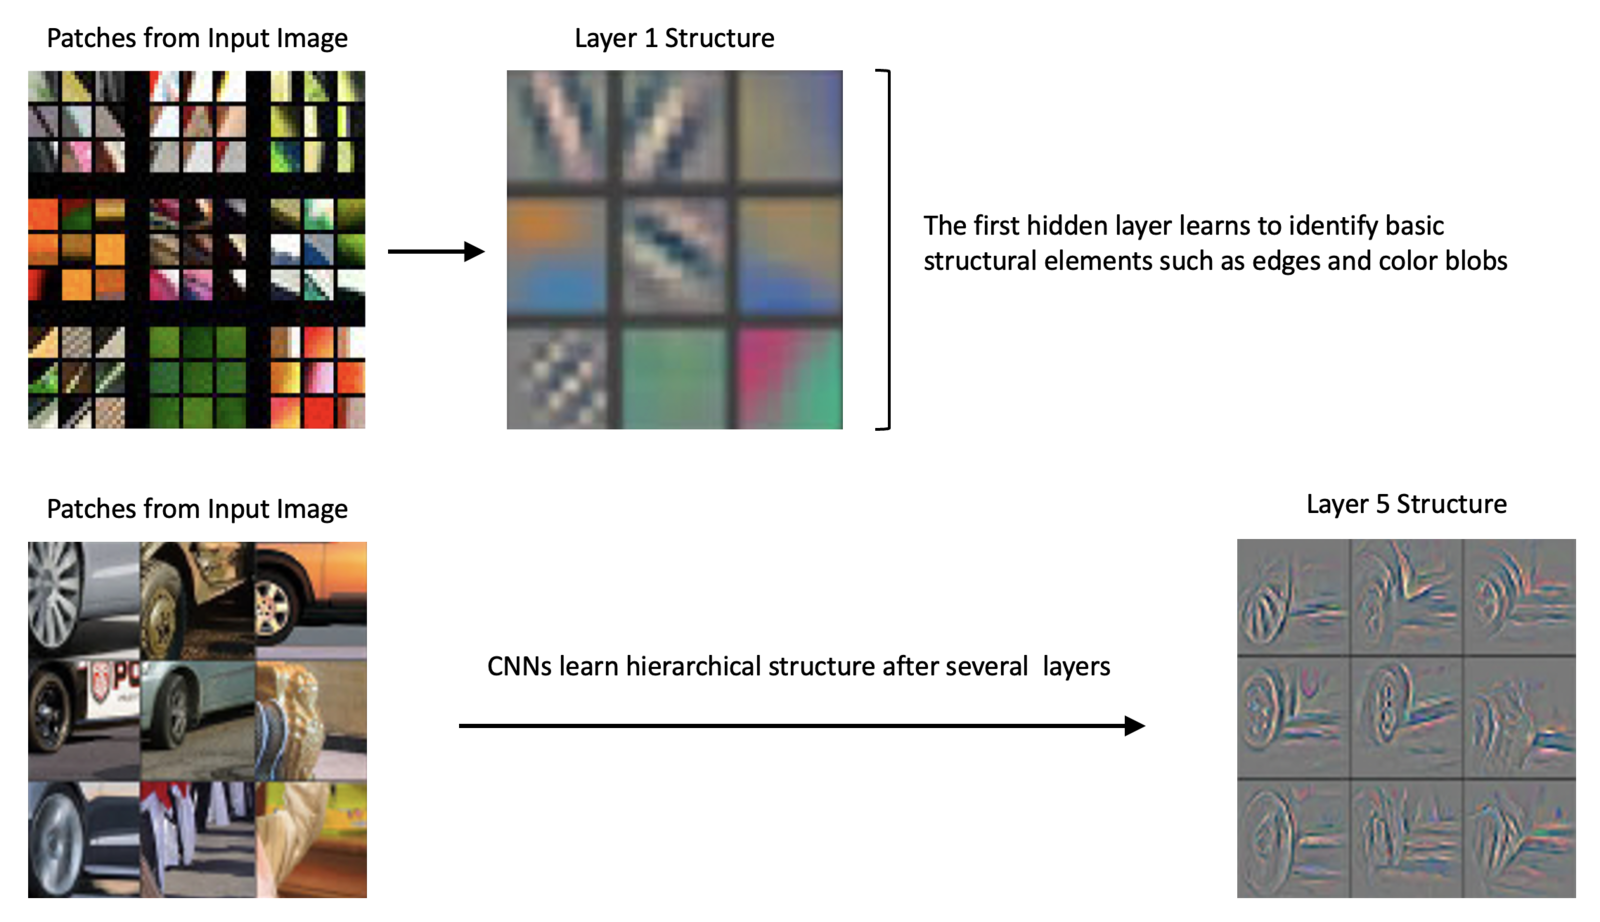
\includegraphics[scale=0.27]{./Images/BA_003_tensorflow-keras-cnn-hierarchical-structure.png}
\caption{Tiefe der Abstraktion von Merkmalen [3]}
\label{Tiefe der Abstraktion von Merkmalen [3]}
\end{figure}

Diese Merkmale sind hierarchisch aufgebaut, das heißt das auf den vorderen Schichten nach Simpleren Formen gesucht wird, und auf den späteren Schichten werden diese Merkmale zu Komplexen Merkmalen zusammengesetzt.

So wie bei den Pooling Layern, werden in den Convolutional Layern Filter eingesetzt, die über das Input Bild gleiten, und eine bestimmte Operation ausführen. Im Gegensatz zu den Pooling Layern, können die Convolutional Layer mehrere Filter besitzen. Dies kann zu Großen mengen an Daten führen, denn jedes Input Bild wird mit jedem Filter verrechnet, und sorgt daher für eine weitere Feature Map. Also die Anzahl der Input Bilder, multipliziert mit der Anzahl der Filter, ergibt die menge der Feature Maps, die an die nächste Schicht weitergegeben werden.

\textbf{Wie Funktioniert die Convolution Operation?}

Die Operation besteht aus einer Rechenoperation zwischen den Filtern, und der Fläche, über welche sie gelegt werden. Ein Filter besteht aus einer Matrix, welche häufig 3x3 oder 5x5 Felder groß ist. 
Ein Filter wird über das Eingangsbild geschoben, so wie bereits bei den Pooling Layern. Allerdings werden hierbei alle Werte mit den Werten des Filters multipliziert, an den Stellen, an denen sie übereinander liegen. Diese Werte werden addiert, und in einer Feature Map gespeichert.
Genau genommen ist diese Operation eine Kreuzkorrelation. Eine Convolution, im Deutschen "Faltung" genannt, wäre eine Kreuzkorrelation, bei der die Filter noch um 180° gedreht werden müssten. Dies ist allerdings nicht nötig für das Netzwerk. Der Name Convolutional Network ist geblieben, aber statt der eigentlichen Faltung wir die Kreuzkorrelation verwendet.
Der Filter kann dabei ganz weit außen starten, oder innerhalb der grenzen des Eingangsbildes. Wenn der Filter ganz weit außen startet, so dass nur ein einziges Feld mit dem Eingangsbild überlappt, dann nennt man das eine "Full Cross-Correlation". Wenn der Filter ganz in der Oberen Linken Ecke startet, dabei aber bereits beim ersten Schritt alle Felder des Filters innerhalb der grenzen des Eingangsbildes befinden, dann nennt man das "Valid Cross-Correlation".
In diesem Netzwerk wird die Valid Cross-Correlation verwendet. Die Größe der entstehenden Feature Map hängt ebenfalls davon ab, welche Cross-Correlation verwendet wird. 
Bei der Full Cross-Correlation wird außerhalb der Matrix angefangen. Das bedeutet, dass mehr Schritte benötigt werden, um durch eine Reihe zu iterieren, und daher entstehen auch mehr Einträge in der Feature Map.

% Done Hier muss noch ein Bild hin welches die Full Cross-Correlation erklärt
\begin{figure}[H]
\centering
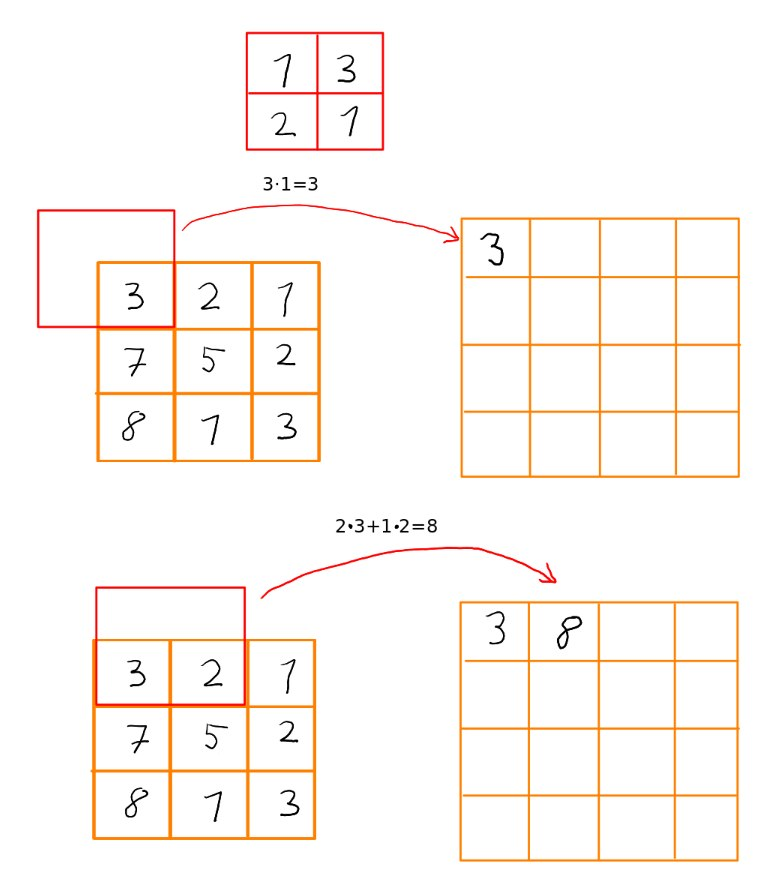
\includegraphics[scale=0.5]{./Images/Full_Correlation_004.jpg}
\caption{Full Cross-Correlation}
\label{Full Correlation}
\end{figure}
 
Die Valid Cross-Correlation hingegen beweg sich nur in den Grenzen des Eingangsbildes, daher entstehen weniger Einträge in die Feature Map.

% Done Hier muss noch ein Bild hin welches die Valid Cross-Correlation erklärt
\begin{figure}[H]
\centering
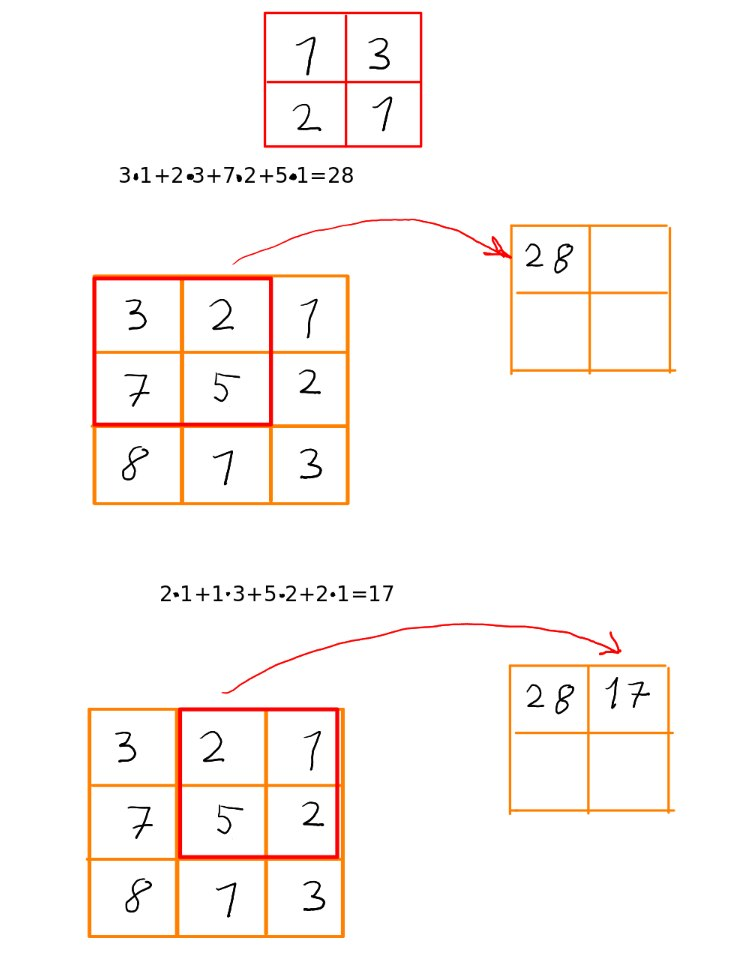
\includegraphics[scale=0.5]{./Images/Valid_Correlation_005.jpg}
\caption{Valid Cross-Correlation}
\label{Full Correlation}
\end{figure}

Die Berechnung der Breite und Höhe einer entstehenden Feature Map sind genauso aufgebaut wie zuvor bei den Pool Layern:

$$H_{out} = (H - filter\_height)/stride + 1$$
$$W_{out} = (W - filter\_ width)/stride + 1$$


% TODO Hier müssen mehr erklärungen hin zu der Funktionsweise der Schicht










\cleardoublepage
\subsection{Forward Propagation im Convolutional Layer}
Grundlegend braucht diese Schicht Filter. Die Filter werden von zwei Parametern gebildet, und zwar "filterSize" und "numFilters". Die Größe der Filter wird dabei von "filterSize" festgelegt, und "numFilters" beschreibt die Anzahl an Filtern. Wir gehen davon aus, dass die Filter immer Quadratisch sind, daher reicht ein Wert um die Größe zu beschreiben.

Darüber hinaus wird wie bei den Pool Layern zuvor, wieder Schritt Größen, also "stepSize", gebraucht. Diese entscheiden, wie viele Pixel der Filter bei einem Schritt überspringt. Wenn diese Größer angelegt werden, werden die Feature maps dementsprechend kleiner, allerdings kann das dazu führen, dass Features nicht erkannt und weiterverarbeitet werden. 

Die Restlichen Werte die übergeben werden haben mit der Verarbeitung der eingangs- und Ausgangsbildern zu tun.

Wichtig ist, dass genau wie in den Fully Connected Layern die anpassbaren Werte nicht mit 0 als Startwert initiiert werden, sondern mit zufällig generierten Zahlen. Ansonsten würden die Anpassungen auch immer gleich aussehen. Die Werte, die in dieser Schicht trainiert werden können, sind die Werte in den Filtern.

Hier ist die Constructor Methode der Klasse "ConvolutionLayer":

\begin{lstlisting}[language=Java]
public ConvolutionLayer(int filterSize, int stepSize, int inLength, int inRows, int inCols, int numFilters, double learnRate) {
        this.filterSize = filterSize;
        this.stepSize = stepSize;
        this.inLength = inLength;
        this.inRows = inRows;
        this.inCols = inCols;
        this.learnRate = learnRate;

        generateRandomFilters(numFilters);
    }
\end{lstlisting}

Und in der Methode "generateRandomFilters" werden die Filter generiert, und mit Zufallszahlen initiiert. Dabei werden die Filter entsprechend der "filterSize" angelegt und die Liste, welche die Filter enthält ist so groß, wie durch "numFilters" angegeben.

\begin{lstlisting}[language=Java]
private void generateRandomFilters(int numFilters) {
        List<double[][]> filters = new ArrayList<>();
        Random random = new Random();

        for (int n = 0; n < numFilters; n++) {
            double[][] newFilter = new double[filterSize][filterSize];

            for (int i = 0; i < filterSize; i++) {
                for (int j = 0; j < filterSize; j++) {
                    double value = random.nextGaussian();
                    newFilter[i][j] = value;
                }
            }
            filters.add(newFilter);
        }
        this.filters = filters;
    }
\end{lstlisting}

Die entstandenen Filter werden in einer Liste gespeichert. Die Objektvariablen sehen ähnlich wie in den anderen Schichten so aus:

\begin{lstlisting}[language=Java]

public class ConvolutionLayer extends Layer {

    private List<double[][]> filters;
    private int filterSize;
    private int stepSize;

    private int inLength;
    private int inRows;
    private int inCols;
    private double learnRate;

    private List<double[][]> lastInput;

\end{lstlisting}









\cleardoublepage
\section{Unterstützungs Templates}
Die Gliederung dieser Arbeit, entspricht einer organischen Herangehensweise oder einer Anleitung, wie ein Netzwerk aufgebaut wird. Jedes Kapitel entspricht einem Teil des Netzwerkes, also den Funktionen, der Initialisierung, der Query oder Abfrage und dem Lern- oder Backpropagation-Algorithmus. Jedes der Kapitel startet mit einer Übersicht, über die Funktionalität, erläutert die Theorie dahinter, teilweise auch mathematisch, und schließt, mit dem daraus resultierenden Code ab. 


\begin{figure}[H]
\centering
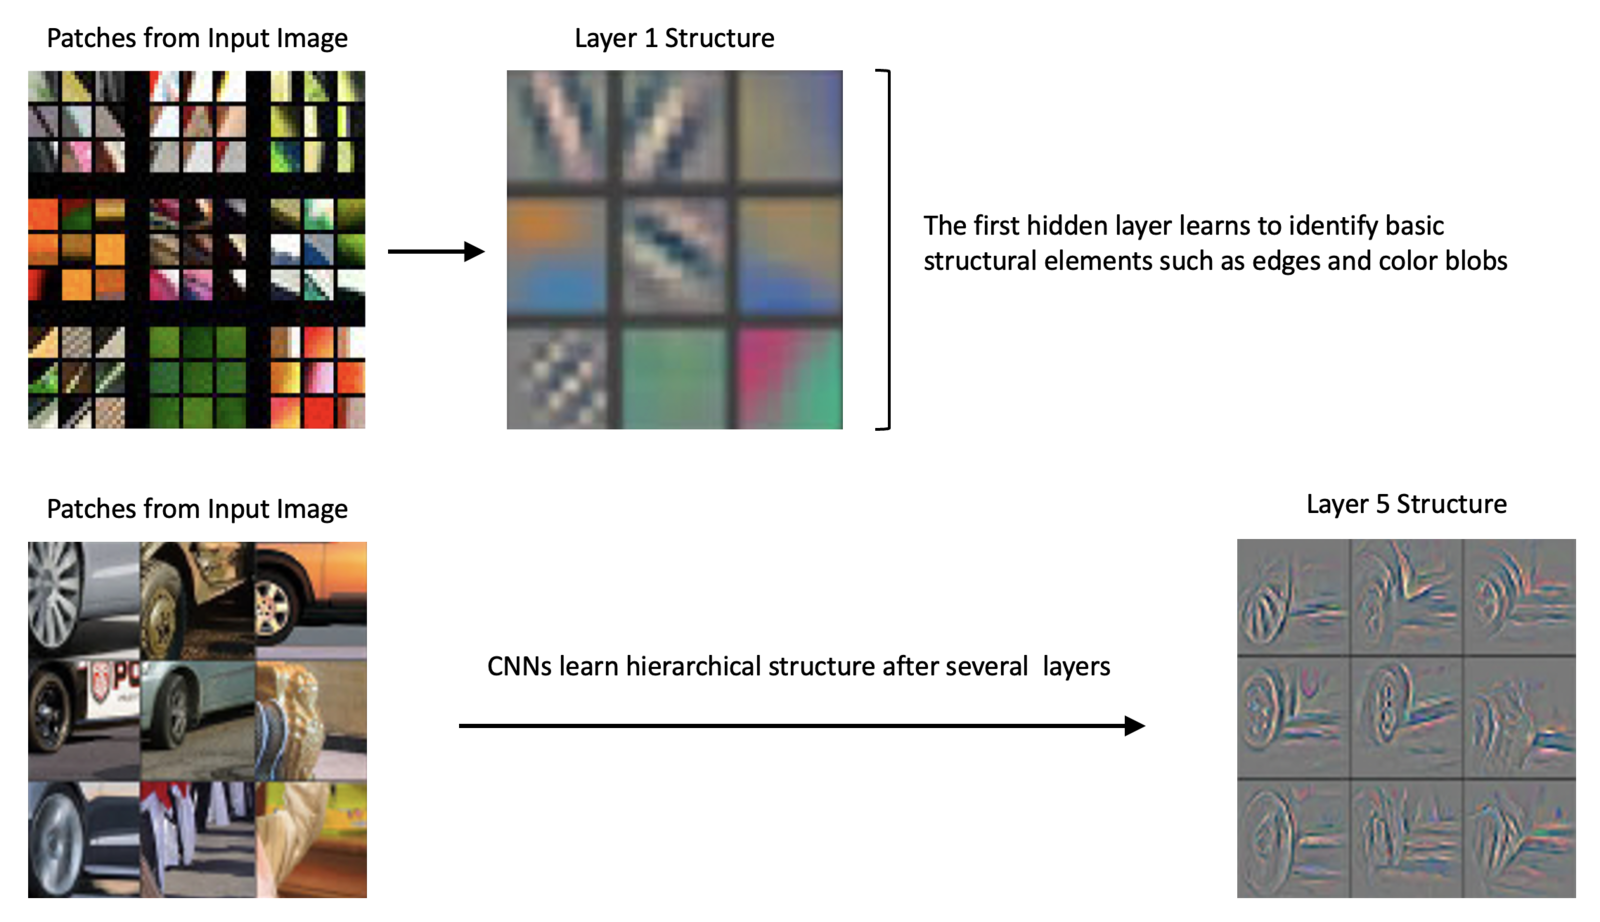
\includegraphics[scale=0.27]{./Images/BA_003_tensorflow-keras-cnn-hierarchical-structure.png}
\caption{Tiefe der Abstraktion von Merkmalen [3]}
\label{Tiefe der Abstraktion von Merkmalen [3]}
\end{figure}


\begin{itemize}
  \item Dendriten
  \item der Zellkörper
  \item das Axon
\end{itemize}

\begin{lstlisting}[language=Java]
public class NeuralNetwork {
    Layer[] layers;
    }
}
\end{lstlisting}

$h$ kürzen:
$$\frac{\Delta e}{\Delta w}=w+w+h$$
$$\frac{\Delta e}{\Delta w}=2w+h$$Und jetzt zum Interessanten Teil. Da wir $h$ nicht gleich 0 setzten können, können wir allerdings $h$ gegen 0 laufen lassen, dann verwenden wir die Leibniz-Notation. Das bedeutet, dass wir anstatt  $\Delta w$ und  $\Delta e$, wobei $\Delta$ eine sehr kleine Vergrößerung darstellt, jetzt $dw$ und $de$ verwenden, wobei $d$ für eine unendlich kleine Vergrößerung steht, eine sogenannte Infinitesimalzahl.
Das sieht dann ungefähr so aus:
$$\frac{de}{dw}=\lim_{h\to 0} 2w +h$$
$$\frac{de}{dw}=2w$$


\section{Einleitung}
\subsection{Motivation}
Neuronale Netzwerke werden vor allem für Klassifikationsverfahren verwendet. In der Praxis gibt es viele Anwendungsbereiche, in denen es vorteilhaft ist, große Mengen von Daten automatisch zu klassifizieren. Einige Beispiele, wären die Bild- und Schrifterkennung, die man dazu verwendet, Kennschilder von Autos, maschinell auszulesen. Solche Technologien werden immer häufiger auf Parkplätzen und Autobahnen eingesetzt. Aber, auch fast jedes Handy kann mittlerweile Schrift erkennen, die mit der Kamera aufgenommen wird. Auch in der Medizin, beim Auswerten von Röntgenbildern, in der Biologie, zum Erkennen von Pflanzen auf Fotos und noch vielem mehr, werden Neuronale Netzwerke inzwischen eingesetzt.\\

\cleardoublepage
% \phantomsection
\sloppy
\section{Quellen}
\begin{itemize}
\item 1. B. Lenze, Einführung in die Mathematik neuronaler Netze. Berlin: Logos Verlag; 2009.
\item 2. Alexey Kravets (02.03.2024), "Forward and Backward propagation of Max Pooling Layer in Convolutional Neural Networks", URL: https://towardsdatascience.com/forward-and-backward-propagation-of-pooling-layers-in-convolutional-neural-networks-11e36d169bec
\item 3. Bill Kromydas (08.03.2024), "Understanding Convolutional Neural Network (CNN): A Complete Guide", URL: https://learnopencv.com/understanding-convolutional-neural-networks-cnn/



\item 4. "Ableitung der Sigmoid-Funktion" URL: \url{https://ichi.pro/de/ableitung-der-sigmoid-funktion-91708302791054}
\item 5. "What is the role of the bias in neural networks?" URL: \url{https://stackoverflow.com/questions/2480650/what-is-the-role-of-the-bias-in-neural-networks}.
\item 6. "How do I choose the optimal batch size?", URL: \url{https://ai.stackexchange.com/questions/8560/how-do-i-choose-the-optimal-batch-size}
\end{itemize}

\cleardoublepage
\section{Liste der Abbildungen}
\listoffigures
\end{document}